% Everything on a line after the symbol % is a comment

%The document class defines the look and feel of the document
%Most of the times, you would use wither an article or a letter class
\documentclass[12pt]{article}

%This package enables the insertion of images into the document
\usepackage{graphicx}

%Enables AMS fonts and other useful commands
\usepackage{amsfonts}
\usepackage{amsmath,amssymb,amsthm}

%This sets 1.2-line spacing between the lines
\renewcommand{\baselinestretch}{1.2}

%These lines set margins, page size, etc. I don't remember
%most of them and use Google when I need to change anything
\setlength{\topmargin}{-0.7in}


\setlength{\textwidth}{6.5in}
\setlength{\oddsidemargin}{0.0in}
\setlength{\textheight}{9.1in}
\newlength{\pagewidth}
\setlength{\pagewidth}{6.5in}
\pagestyle{empty}




%These define 'custom commands'. Mostly, these are simply
%shortcuts for longer commands. The syntax is
%\def\blah{\longlonglongcommand}
%This means you would type \blah instead of \longlonglongcommand

%Paragraph without indentation
\def\pp{\par\noindent}

%Empty set
\def\O{{\varnothing}}

%=>
\def\>{{\Rightarrow}}

%Reals
\def\rr{\mathbf{R}}

%Rationals
\def\qq{\mathbf{Q}}


%Naturals
\def\nn{\mathbf{N}}

%Positive integers
\def\zz{\mathbf{Z^+}}

%emptyet
\def\ES{{\varnothing}}

%arrows
\def\>{{\Rightarrow}}
\def\=>{{\Rightarrow}}
\def\->{{\rightarrow}}
\def\M->{{\mapsto}}


\def\e{\exists}
\def\ne{\notexists}
\def\st{such that}
\def\s{\Sigma}
\def\d{\delta}
\def\e{\epsilon}

% |
\def\|{\mid}

%<=>
\def\lr{{\Leftrightarrow}}

%these are shortcuts for environment elements
\def\nums{\begin{enumerate}}
\def\nume{\end{enumerate}}
\def\x{\item}

%I have borrowed the following code from somebody. Note the usage later!

\newtheorem{theorem}{Theorem}[section]
\newtheorem*{theorem*}{Theorem}
\newtheorem{lemma}[theorem]{Lemma}
\newtheorem{proposition}[theorem]{Proposition}
\newtheorem{corollary}[theorem]{Corollary}
\newtheorem{exercise}[theorem]{Exercise}
\newenvironment{definition}[1][Definition]{\begin{trivlist}
\item[\hskip \labelsep {\bfseries #1}]}{\end{trivlist}}
\newenvironment{example}[1][Example]{\begin{trivlist}
\item[\hskip \labelsep {\bfseries #1}]}{\end{trivlist}}
\newenvironment{remark}[1][Remark]{\begin{trivlist}
\item[\hskip \labelsep {\bfseries #1}]}{\end{trivlist}}
\newenvironment{answer}[1][Answer]{\begin{trivlist}
\item[\hskip \labelsep {\bfseries #1}]}{\end{trivlist}}
\newenvironment{solution}[1][Solution]{\begin{trivlist}
\item[\hskip \labelsep {\bfseries #1}]}{\end{trivlist}}

\setcounter{secnumdepth}{-1} 

\setlength{\parindent}{0in}

\usepackage{abstract}
\renewcommand{\abstractname}{}    % clear the title
\renewcommand{\absnamepos}{empty}


%Now let's enter data for the title page
\title{MAT 312 / AMS 351 final exam}
\date{August 16, 2012}
\begin{document}
\maketitle 
Name:

SBU ID:
\\
\\
Please do not ``show work"; write your work on the backs of the pages. It is not graded.  Instead, after solving a problem, write the solution in the form of a series of concise sentences or computations. These should appear in a logical order rather than the order in which you thought of them.
For example, to present the fact that the number $x=4$ satisfies the equation $x+3=7$, the following is not acceptable:

\begin{align*}
x+3=7 \\
x+3-3=7-3 \\
x=4
\end{align*}

Instead, you would write something like:

If $x=4$, then $x+3=4+3=7$.  Then this $x$ solves the equation $x+3=7$.
\\
\\
No cheating.
\newpage
\begin{enumerate}
\item
Use the Euclidean algorithm to:\begin{enumerate}
\item find the greatest common divisor of 1000 and 105
\item find two integers $s$ and $t$ such that $1000s+105t=5$, and
\item list two integers that are inverses for $21$ modulo $200$.
\end{enumerate}
\newpage
\item
Find an integer $x$ such that
\begin{align*}
(\operatorname{mod} 1000) 105x\equiv 10
\end{align*}
\newpage
\item
Compute all of the powers of $[2]_{30}\in \mathbb{Z}_{30}$.  Find an integer congruent to $2^{902}$ (using the modulus 30).

\newpage
\item
Find two integers $y$ such that
\begin{align*}
y\equiv 0 \operatorname{mod}200\\
y\equiv 5 \operatorname{mod}21
\end{align*}
\newpage
\item
Recall that for a positive integer $n$, the Euler function $\phi(n)$ is by definition the number of elements $[x]_n$ of $\mathbb{Z}_n$ that have multiplicative inverses (that is, those that satisfy $\operatorname{gcd}(x,n)=1$).  It can be computed in terms of the prime factorization for $n$ by
\begin{align*}
\phi({p_1}^{a_1}{p_2}^{a_2}...{p_k}^{a_k})=(p^{a_1}-p^{a_1-1})(p^{a_2}-p^{a_2-1})...(p^{a_k}-p^{a_k-1})
\end{align*}
\begin{enumerate}
\item
Compute $\phi(21)$
\item
List the elements of $\mathbb{Z}_{21}^{*}$ (the invertible classes).
\item
Show that $[2]_{21}$ has order 6 in the group $\mathbb{Z}_{21}^{*}$
\end{enumerate}
\newpage
\item
You shuffle an 8-card deck perfectly:
\begin{center}
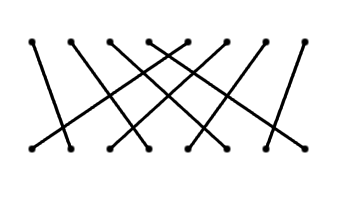
\includegraphics{shuffle.png}
\end{center}
\begin{enumerate}
\item
Write this permutation $\sigma\in S_{8}$ in the cycle notation, as a product of disjoint cycles.  How many times would you have to perform this exact shuffle to return to the original configuration?
\item
Suppose I switched cards 3 and 6 before you shuffle.  What shuffle is accomplished after you do $\sigma$?  Express your answer in cycle notation.
\end{enumerate}
\newpage
\item
Let $S$ be the set of ways of choosing 3 beads in a circle of 6 to be black, so $S$ is:
\begin{center}
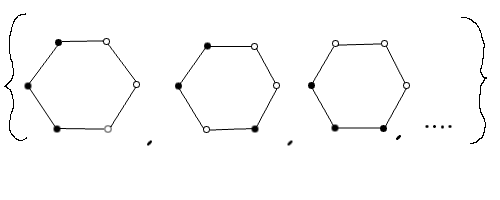
\includegraphics{beads.png}
\end{center}
Notice that $S$ has $\binom{6}{3}=20$ elements.  The group $\mathbb{Z}_6$ acts on this set by rotating.  How many distinct configurations of beads are there?  That is, how many orbits are there for the action of $\mathbb{Z}_6$ on $S$?  Draw a sample of each type of configuration (in addition to the two displayed above).
\newpage
\item
I encrypt an integer between 0 and 4 using your RSA public key with modulus 55 and exponent 27.  You receive 18.  What was my number?
You may use the following facts:
\begin{align*}
18^1=18\\
18^2=324\\
18^3=5832\\
18^4=104976
\end{align*}
\newpage
\item
Part of an infinite planar figure is shown.  On the second diagram:
\begin{itemize}
\item
draw all lines of reflective symmetry with a dotted line
\item
draw all lines of ``only glide symmetry" (lines which are not also lines of reflective symmetry) with solid lines, with at least one darkened interval indicating the amount of the translation part
\item
draw small circles at all points of rotational symmetry, labelled with an integer indicating the order of the rotation (for example, with 2 if $180^{\circ}$)
\item
draw two vectors, somewhere near the bottom of the diagram, generating the translation symmetries
\end{itemize}
\begin{center}
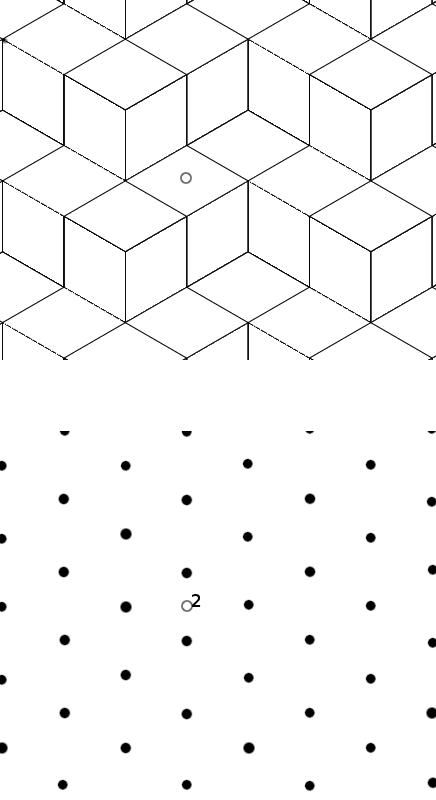
\includegraphics[scale=0.70]{exam.png}
\end{center}
\end{enumerate}
\end{document}
